\section{Musical instruments - basic principles}
\bi

\i This section provides a basic introduction to 
the production of sound by musical instruments.

\i We will consider three stringed instruments 
(the harp, guitar, and violin); 
a three wind instruments 
(organ pipes, a penny whistle, and clarinet);
and two tuned-percussion instruments
(the glockenspeil and piano).

\i The presentation follows that of ``How music works,"
by John Powell.
More details can be found in the text by Berg and Stork.

\ei
%%%%%%%%%%%%%%%%%%%%%%%%%%%%%%%%%%%%%%%%%%%%%%
\subsection{Sounds from strings}
\bi

\i String instruments come in two types: 
those that are bowed and those that are plucked.

\i Examples of bowed string instruments are the 
violin, cello, ...\\
Examples of plucked string instruments are the 
harp, guitar, banjo, ...

%\i Plucking and bowing are the two basic methods
%for exciting vibrations in a stretched string.

\i As discussed in a previous section about 
standing waves, frequency of vibration of a stretched
string depends on only three things:
(i) the length of the string, 
(ii) what the string is made of, and
(iii) the tension in the string.

(i) The length of the string determines how far
the waves have to travel to go from one end to
another.
The longer the string, the longer the travel
time, and hence the lower the frequency of vibration.

(ii) What the string is made of is important 
since heavier strings offer more resistance 
to changes in their state of motion, and hence 
correspond to lower-frequency waves.

(iii) The tension in the string is a measure of 
how tightly the string is stretched.
Strings under higher tension are pulled back toward
their equilibrium position with greater force,
and hence correspond to higher-frequency waves.

\i The mathematical formula for the frequency
of the nth standing wave pattern on a string
is
%
\be
f_n = \frac{n}{2L}\sqrt{\frac{\tau}{\mu}}\,,
\qquad
n=1,2,3,\cdots
\ee
%
where $L$ is the length of the string,
$\mu$ is it mass per unit length, and 
$\tau$ is the tension in the string.
($f_1$ is the fundamental frequency and 
$f_n = nf_1$ is the nth harmonic.)

\ei
%%%%%%%%%%%%%%%%%%%%%%%%%%%%%%%%%%%%%%%%%%
\subsection{Harp}
\bi

\i The harp is probably the simplest of all stringed
instruments.
(See Figure~\ref{f:harp}.)
%
\begin{figure}[htbp]
\begin{center}
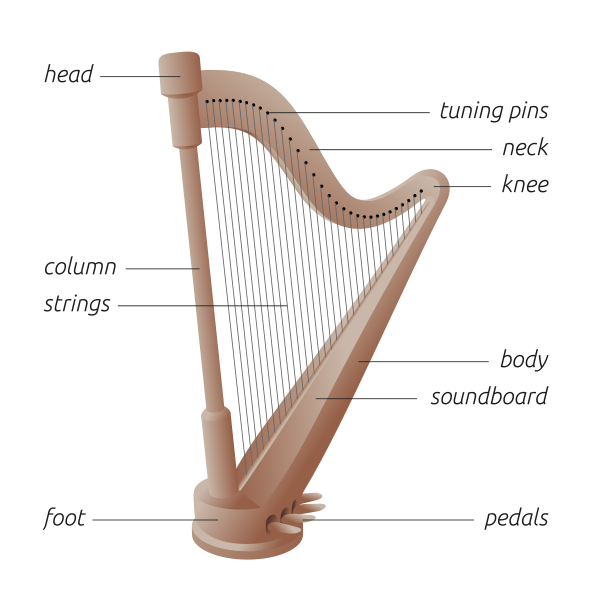
\includegraphics[width=.8\textwidth]{Harp.png}
\caption{The parts of a harp.
(Figure taken from Wikipedia.)}
\label{f:harp}
\end{center}
\end{figure}

\i The strings have fixed lengths and they are 
plucked.

\i Each string produces just one note.
(That's why a harp needs so many strings!)

\i However, by using a foot pedal that changes
the tension in the strings, one can raise or 
lower the note by a semitone.
(A harp with such a foot pedal is called a 
{\em double-action} harp.)

\i Plucking the strings in the middle give the 
purest tones, having contributions from only odd
harmonics.
Plucking the strings near one of the ends 
produces ``fuller" tones, having contributions from
both even and odd harmonics.
(See Figure~\ref{f:pluckedstrings}.)
%
\begin{figure}[htbp]
\begin{center}
\begin{tabular}{cc}
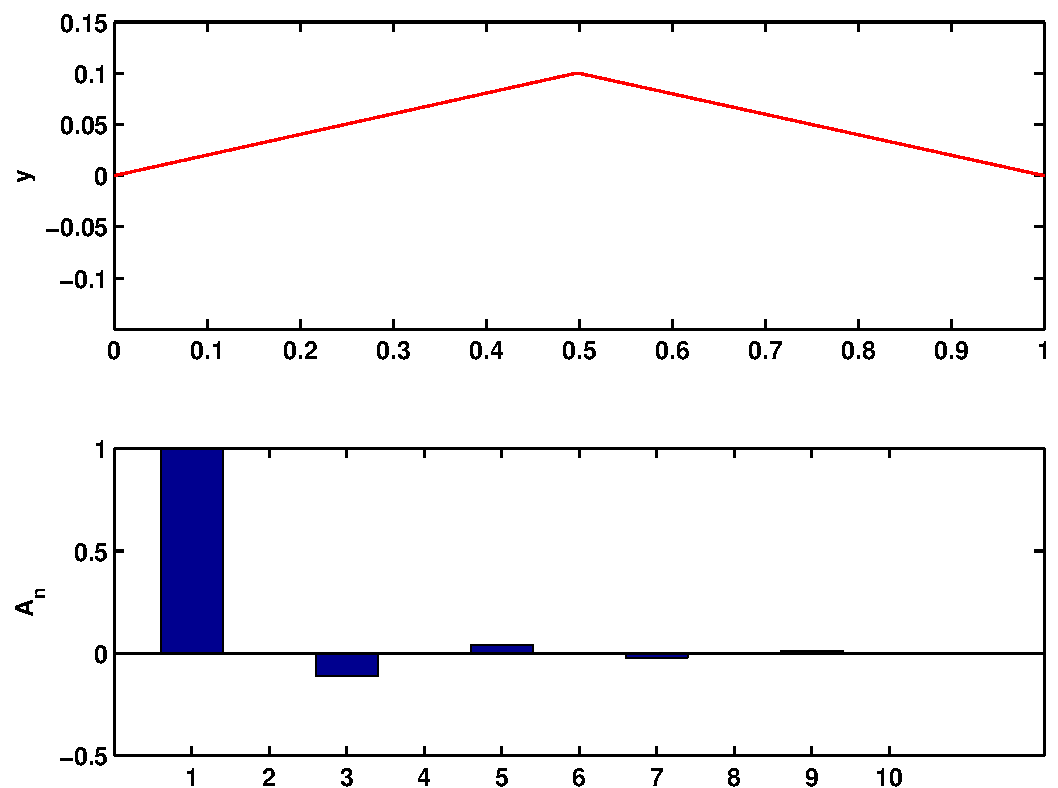
\includegraphics[width=.5\textwidth]{pluckedstringharmonics1_2.pdf} &
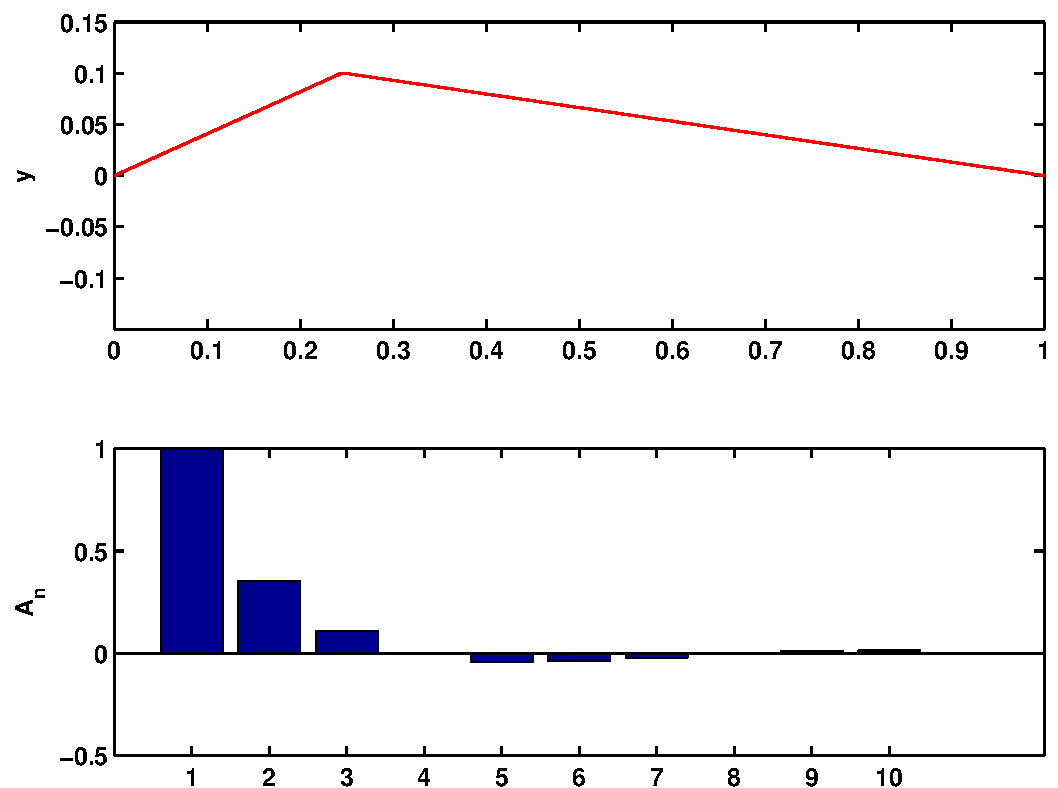
\includegraphics[width=.5\textwidth]{pluckedstringharmonics1_4.pdf}
\\
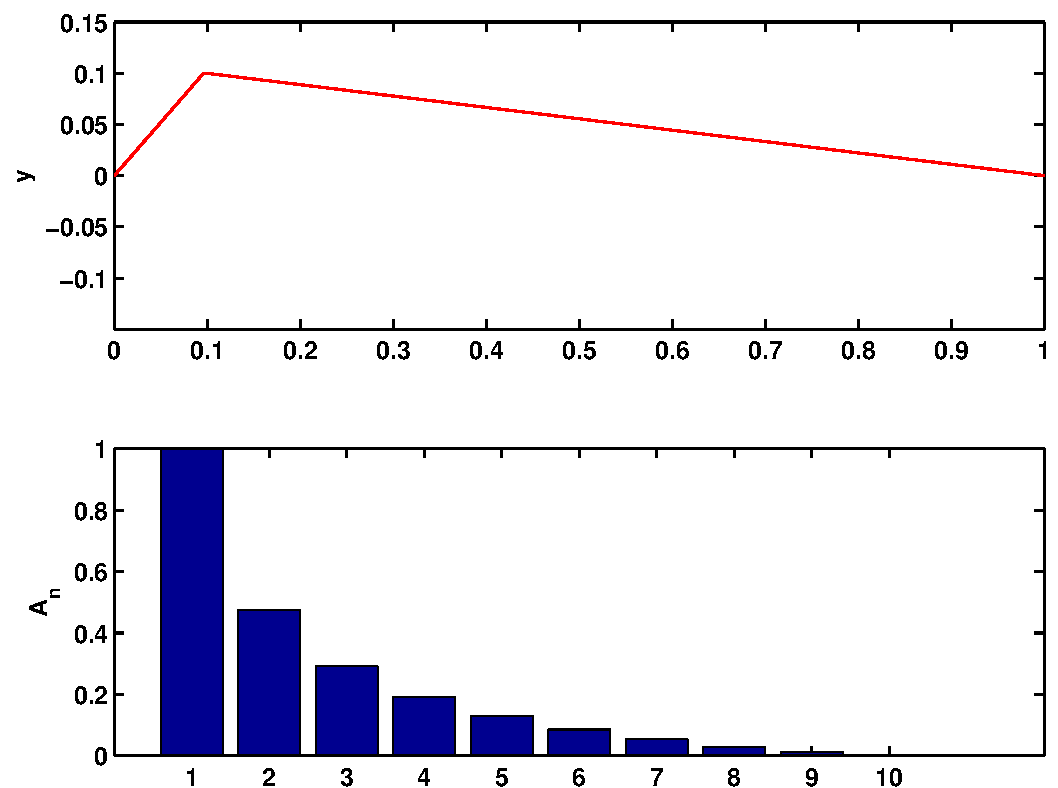
\includegraphics[width=.5\textwidth]{pluckedstringharmonics1_10.pdf} &
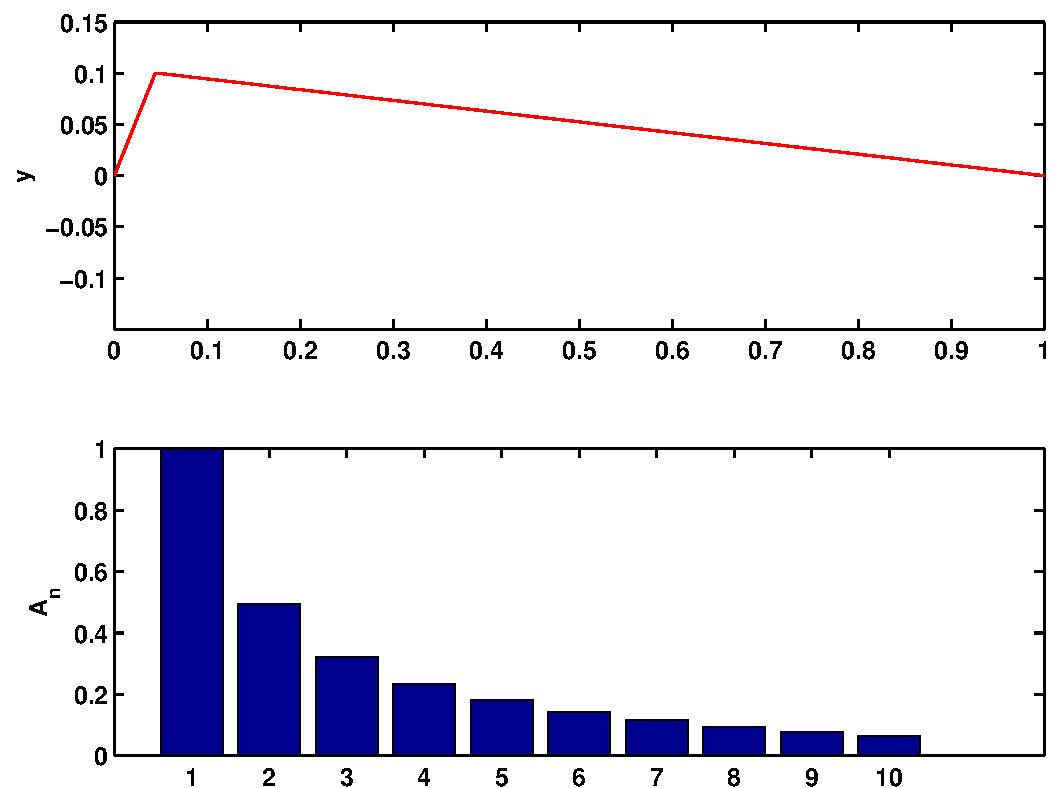
\includegraphics[width=.5\textwidth]{pluckedstringharmonics1_20.pdf} 
\end{tabular}
\caption{Fourier coefficients corresponding to strings
plucked in different locations.
Note that a string plucked in the center (top-left plot)
corresponds to the purest tone, with small contributions 
from the odd harmonics.
A string plucked near the end (bottom-right plot) corresponds
to a fuller sound, with relatively large contributions from 
many harmonics.}
\label{f:pluckedstrings}
\end{center}
\end{figure}

\i \demo Illustrate this using the matlab
routines {\tt pluckedstring.m}.

\i \demo Watch the YouTube videos
{\tt http://www.youtube.com/watch?v=\_X72on6CSL0}
and\\
{\tt  http://www.youtube.com/watch?v=INqfM1kdfUc}.

\i Note that plucking a string a fraction $1/n$ from the
end (where $n$ is a positive integer), does not have 
contributions from the nth harmonic and all its multiples.

\i A vibrating string by itself doesn't produce much 
sound.
The vibrations of the strings are amplified by
attaching them to a wooden box (called a soundboard), 
which is able to drive more air and produce a louder sound.

\ei
%%%%%%%%%%%%%%%%%%%%%%%%%%%%%%%%%%%%%%%%%%
\subsection{Guitar}
\bi

\i The guitar is probably the next simplest string
instrument.
(See Figure~\ref{f:guitar}.)
%
\begin{figure}[htbp]
\begin{center}
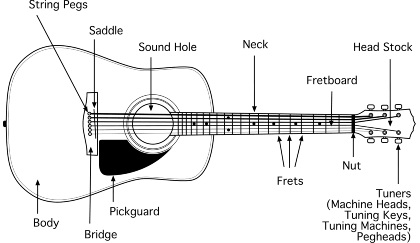
\includegraphics[width=.9\textwidth]{guitar.jpg}
\caption{The parts of a classical guitar.
(Figure taken from {\tt http://www.betterguitar.com}.)}
\label{f:guitar}
\end{center}
\end{figure}

\i It has six strings all of the same length.

\i The strings are made of different materials 
and are under different tensions, to produce notes 
with different pitches.
(The tension in the strings can be adjusted 
using the tuning keys.)

\i By pressing the strings against frets, which
are located on the neck of the guitar (between the
nut and the bridge), the effective lengths of 
the strings can be changed.
This increases the number of notes that can be 
produced.

i) By pressing a string against the seventh fret,
you decrease its length to two-thirds of its full 
length, producing a sound a perfect fifth above
that the open string.

ii) By pressing a string against the twelfth fret,
you decrease its length to one-half of its full
length, producing a sound an octave above that of
the open string.

\i By wiggling your finger on the fret as you
pluck a string, you can produce a note with a 
varying pitch.
This effect is called {\em vibrato} and is used 
a lot by violinists and sometimes vocalists.

\i The strings are coupled to the body of the 
guitar at the bridge.
The vibrations of the strings are amplified by
the body, increasing the loudness of the sound 
produced.

\ei
%%%%%%%%%%%%%%%%%%%%%%%%%%%%%%%%%%%%%%%%%%%
\subsection{Violin}
\bi

\i Although a violin is superficially similar to a guitar, 
it differs from a guitar in many ways.
(See Figure~\ref{f:violin}.)
%
\begin{figure}[htbp]
\begin{center}
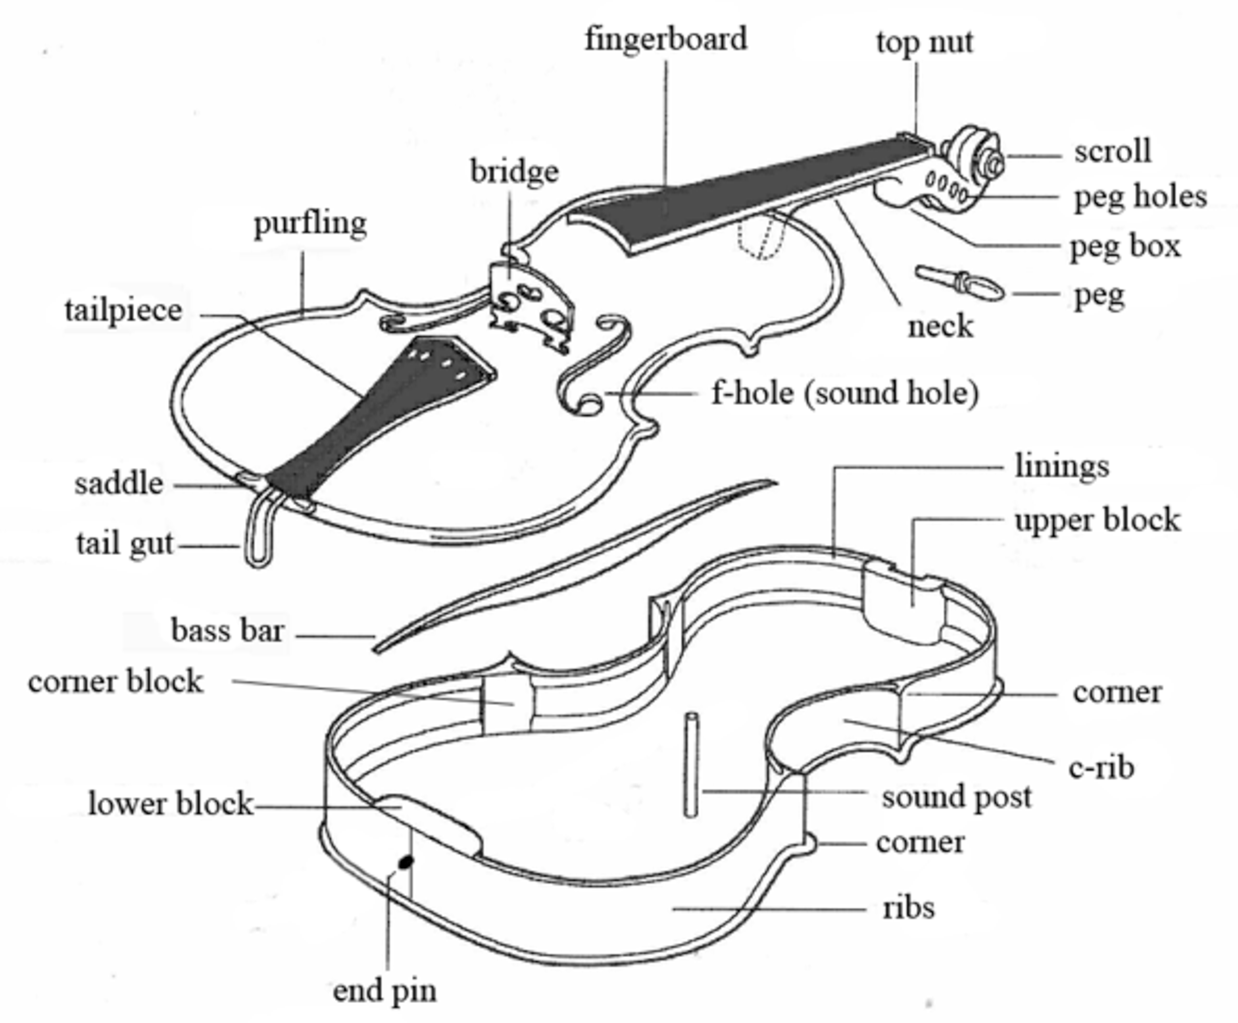
\includegraphics[width=.9\textwidth]{violin.pdf}
\caption{The parts of a violin.
(Figure taken from {\tt http://www.violinsonly.info}.)}
\label{f:violin}
\end{center}
\end{figure}

\i A violin has only four strings of fixed length
and fixed tension.
(Similar to a guitar, 
the tension in the strings can be adjusted
by using the tuning keys.)

\i Similar to a guitar, the effective length of 
the violin strings can be shortened by pressing the 
strings against the neck of the violin.
But unlike a guitar, there are no frets on a violin 
to give fixed, discrete changes in length.

\i Thus, a violin doesn't have fixed notes.
(This makes it harder for a beginner to learn
how to play a violin.)

\i Another major difference between the violin and 
the guitar (or the harp) is that the violin strings 
are typically bowed.

\i A violin bow is typically made from hairs from
a horse's tail, stretched tight on a stick.
The horse hairs are made sticky by rubbing them
with rosin, which is dried tree resin.

\i The bow excites a violin string via an 
alternating {\em stick-slip} motion.
The bow first `sticks' to a string, dragging it 
away from its equilibrium position.
The string then `slips' from under the bow,
as it moves back towards, and then overshoots,
its equilibrium position.
See Figure~\ref{f:stickslip}.
%
\begin{figure}[htbp]
\begin{center}
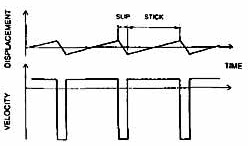
\includegraphics[width=.6\textwidth]{stickslip.jpg}
\caption{Stick-slip motion of a bowed violin string.
Top panel shows string displacement as a function of time.
Bottom panel shows string velocity as a function of time.
This example is for the case where the string is bowed
one-quarter of the way from one of the ends of the string.
(Figure taken from {\tt http://www.zainea.com/}.)}
\label{f:stickslip}
\end{center}
\end{figure}

\i This happens hundreds of times per second, 
corresponding to the natural vibrational frequency 
of string.

\i \demo 
Wet your finger and rub it across a window pane 
or rim of a glass.
Your finger tip slips and sticks as you press 
your finger against the glass, producing a 
squeaking sound as it moves.

\i The vibrational motion of a bowed violin 
string consist consists basically of a kink in 
the string which moves either counter-clockwise
(or clockwise) around the string from bridge
to nut and back to the bride as shown in 
Figure~\ref{f:violinbowed}.
Counter-clockwise motion corresponds to 
upward motion of the bow; 
clockwise motion corresponds to downward motion
of the bow.
%
\begin{figure}[htbp]
\begin{center}
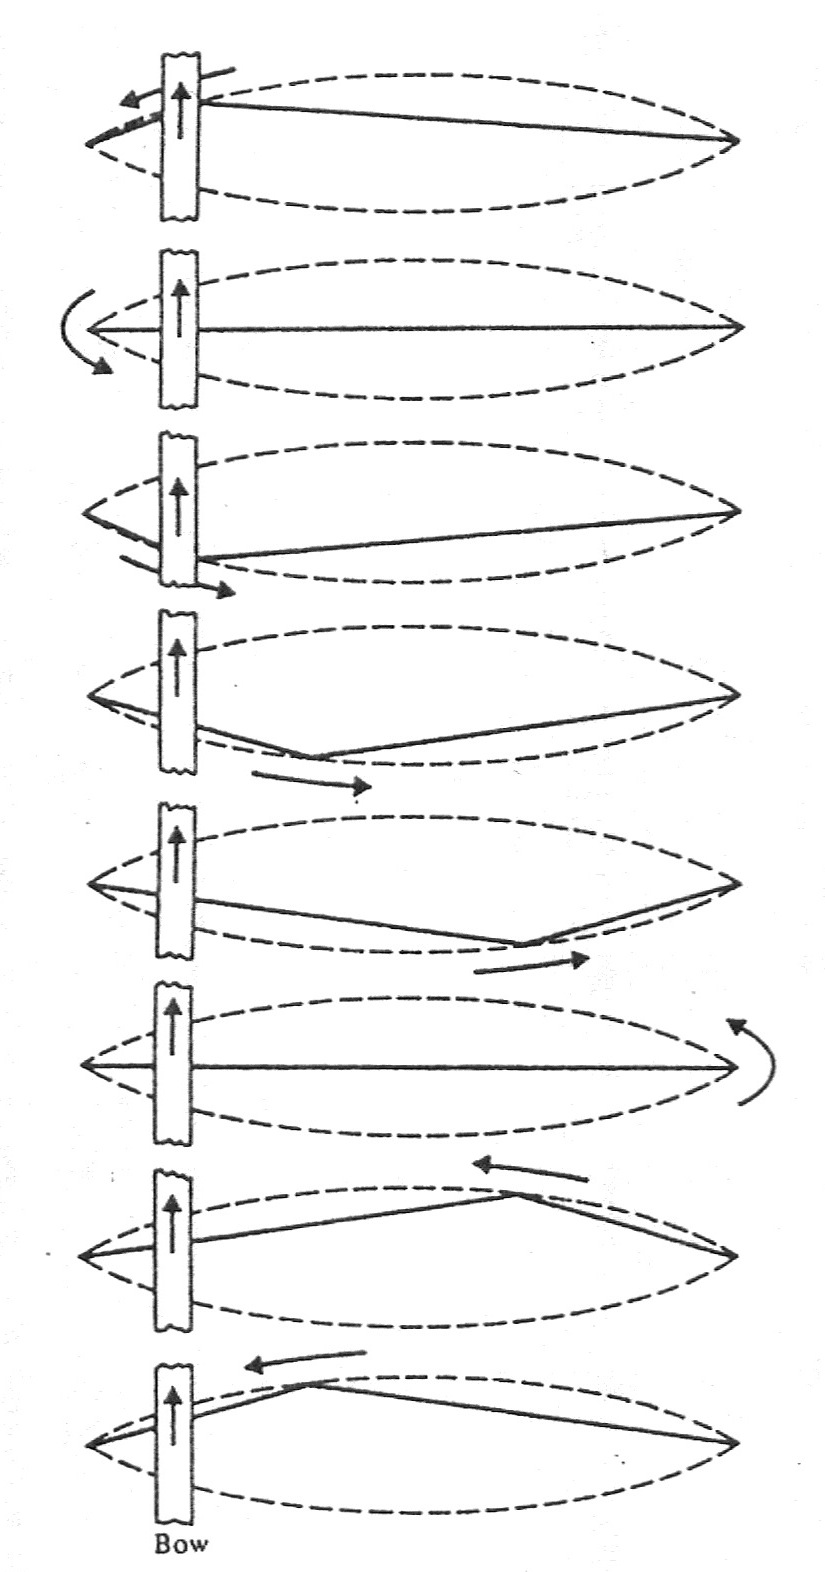
\includegraphics[height=.8\textheight]{violinbowed.jpg}
\caption{Schematic diagram showing the motion of a bowed violin string.
In the top three panels, the string slips from underneath 
the bow, with the kink traveling counter-clockwise
from bow to bridge to bow again.
In the bottom five panels, the string sticks to the bow 
and is dragged along with it, with the kink traveling 
counter-clockwise from bow to nut, and eventually back to 
the bow again.
(Figure taken from {\tt http://www.colorado.edu/physics/phys1240/}.)}
\label{f:violinbowed}
\end{center}
\end{figure}

\i \demo Illustrate this with the matlab routine
{\tt bowedstring.m}.

\i \demo
Watch the YouTube video
{\tt http://www.youtube.com/watch?v=6JeyiM0YNo4}.

\i {\em All} harmonics of the vibrating string are 
excited by  the bowing motion, 
{\em regardless of the location of the bowing}.
The Fourier coefficients have the form
$(-1)^{n+1}/n^2$, independent of the location of
bowing.

\i This is in contrast to the harp or guitar, where 
plucking a string in different locations excites different
combinations of harmonics.
The Fourier coefficients for a plucked string have the form
$\sin(n\pi\alpha)/n^2$, where $\alpha$ is the fraction
of the total length of the string where it is plucked.

\i Note:
The above statements about bowing are strictly true 
for bowing motion perpendicular to the direction of 
the string, and for a very narrow bow.
Since real bows have a considerable width, 
the kink in the waveform is smoothed out, eliminating
some the higher harmonics.
Thus, in practice there is a slight dependence of 
the harmonics on the location of bowing.

\i The tone quality of a violin note can be varied by 
varying the strength of a note as a string is being bowed.
 
\i This is in contrast to the  harp, guitar, or piano, 
where once a string is plucked, nothing else can be
done to change the strength of the note as the string vibrates.
 
\i The strings are coupled
to the body of violin at the bridge
(just like a guitar) and also via the 
sound post (which couples the front and back
of the body).

\i There is a sideways force on the bridge exerted
by the motion of the string.
In the limit of an infinitesimally narrow bow, this
force has the shape of a sawtooth wave, independent
of the location of the bowing.
The Fourier coefficients of the sawtooth wave
have the form $(-1)^{n+1}/n$.

\i For a plucked string, the sideways force on 
the bridge has the shape of a square wave.
The durations of the positive and negative parts
of the square wave are proportional to the 
fraction of the total length of the string where 
the string is plucked.
The Fourier coefficients of the square wave 
have the form $\sin(n\pi\alpha)/n$.

\i \demo Illustrate these two statements with the 
matlab routines 
{\tt bowedstring.m} and
{\tt pluckedstring.m}.

\i The sound hole of a violin (two $f$-holes)
is much smaller than the sound hole of a guitar.

\i The complicated shape of the violin and 
the use of a bow are responsible for the rich
timbre or tone quality of a note played on
a violin.

\ei
%%%%%%%%%%%%%%%%%%%%%%%%%%%%%%%%%%%%%%%%%%%%%%
\subsection{Sounds from wind in tubes}
\bi

\i As discussed in a previous section about 
standing waves, it is possible to create 
vibrations in a column of air in a tube which 
is either open at both ends, or open at one end
and closed at the other.

\i The source of excitation for the vibrating
air column can be either an 
{\em oscillating air jet} 
(like that from a whistle) or a 
{\em vibrating reed} 
(for a clarinet, reed organ pipe, ...) or the
{\em vibrating lips} of a brass player.

\i The oscillating air jet is an example of 
a {\em flow-controlled} excitation, while that of
a vibrating reed (or vibrating lips) is an 
example of a {\em pressure-controlled} excitation.

\i For both of these scenarios, the frequency 
of vibration of the air jet or the reed 
(or lips) is then selected by a resonance process, 
determined by the natural frequencies of the
air column in the tube.  
Recall that the natural frequencies of the air
column in the tube depend only on two things:
(i) the length of the tube, and (ii) whether it 
is closed at one or open at both ends
(in addition the speed of sound in air).

\i Mathematically, the frequency of the nth 
standing wave vibration of the air column
in a cylindrical tube of length $L$ is given by:

Tube open at both ends:
%
\be
f_n = n\left(\frac{v}{2L}\right)\,,
\qquad
n=1,2,3,\cdots
\label{e:open}
\ee
%
Tube open at one end, closed at the other:
%
\be
f_n = n\left(\frac{v}{4L}\right)\,,
\qquad
n=1,3,5,\cdots
\label{e:closed}
\ee
%

\i In these formulae, $v$ is the speed of sound in air 
($v=343~{\rm m/s}$ at room temperature).

\i We will also assume that the tubes are sufficiently
narrow so that end effects are not important.
Otherwise, we would have to increase the effective 
length of the tube by $0.61 R$ for each open end,
where $R$ is the radius of the tube.

\i Note that for tubes closed at one end,
only odd harmonics are present.
Tubes open at both end have both even and odd 
harmonics.

\i We will see below that wind instruments that
use reeds or depend on the vibrating lips of the 
player behave like tubes that are closed at one end.

\i Examples of wind instruments that have reeds 
are the clarinet, bassoon, oboe, ...\\
Examples of wind instruments that don't have reeds
are the flue-organ pipe, penny whistle, flute, ...

\ei
%%%%%%%%%%%%%%%%%%%%%%%%%%%%%%%%%%%%%%%%%%%%%%
\subsection{Flue-organ pipes}
\bi

\i The excitations of the vibrating air 
column in a flue-organ pipe are driven by an
oscillating air jet as shown in 
Figure~\ref{f:fluepipe}.
%
\begin{figure}[htbp]
\begin{center}
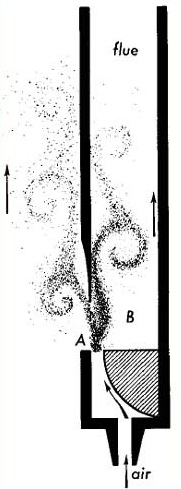
\includegraphics[width=.3\textwidth]{fluepipe.jpg}
\caption{Schematic diagram showing air flow
in a flue-organ pipe.
(Figure taken from {\tt http://home.comcast.net}.)}
\label{f:fluepipe}
\end{center}
\end{figure}

\i When an organ key is depressed, a constant 
flow of air is directed toward a sharp edge
at one end of the organ pipe.
The flow doesn't simply divide evenly on each
side of the edge; 
instead, whirpools (or eddies) are created, 
which take turns going to one
side or the other of the sharp edge.
This is analogous to cars in traffic deciding
to go to either one side or the other of 
a divider in the road, based on the choice of
the previous cars.

\i The frequency with which the whirlpools
are formed on opposite sides of the edge
is determined by the natural frequencies of the
section of pipe above it.
A resonance condition is set up when the 
frequency of whirpool formation matches one
of the natural frequencies of the organ pipe.

\i Since the whirpools are associated with
air molecule motion, the location of the 
sharp edge is an {\em anti-node} for air molecule 
displacement (or a node for pressure deviation), 
and thus corresponds to an {\em open} end of a tube.
If the other end of the organ pipe is open, 
then Equation~\ref{e:open} 
should be used for the natural frequencies.
If the other end of the organ pipe is closed, 
then Equation~\ref{e:closed} should be used.

\i This is the basic operation of a 
whistle, or producing a sound by blowing
over a bottle.

\i \ex
For a bottle shaped like that in 
Figure~\ref{f:helmholtzresonator}
the natural frquency is given by
%
\be
f = \frac{v}{2\pi}\sqrt{\frac{A}{Vl}}
\ee
%
where $l$ is the length of the neck, $A$ is its
cross-sectional area, $V$ is the volume of 
the base, and $v$ is the speed of sound in air.
%
\begin{figure}[htbp]
\begin{center}
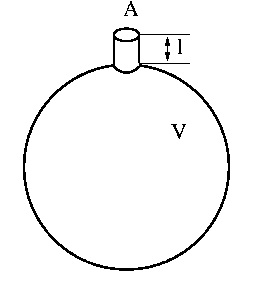
\includegraphics[width=.4\textwidth]{helmholtzresonator.jpg}
\caption{Schematic diagram of a simple
bottle-like resonator.
(Figure taken from {\tt http://fisicaondemusica.unimore.it}.)}
\label{f:helmholtzresonator}
\end{center}
\end{figure}

\i \demo
Calculate the resonant frequency of a bottle,
approximating the neck length, surface area,
and volume.
Blow over the lip of the bottle to produce a sound, and
use iSpectrum to determine its fundamental frequency.
How well does the calculated frequency agree 
with measured frequency?

\i There are also reed-organ pipes, where
the sharp edge of the pipe is basically replaced 
by a vibrating reed.
The operation of such pipes is similar to 
that of a clarinet, which we will talk about 
in a later section.

\ei
%%%%%%%%%%%%%%%%%%%%%%%%%%%%%%%%%%%%%%%%%%%%%%
\subsection{Penny whistle}
\bi

\i A penny whistle is like an organ pipe but with 
a series of holes drilled in it.

\ei
%%%%%%%%%%%%%%%%%%%%%%%%%%%%%%%%%%%%%%%%%%%%%%
\subsection{Clarinet}
\bi

\i The action of the reed is similar to that of 
a bow for a violin.

\i Natural frequency of reed approximately that
of the clarinet pipe.

\i In cylindrical pipes, only odd harmonics are heard.
For conical pipes, both even and odd harmonics
are present.

\ei
%%%%%%%%%%%%%%%%%%%%%%%%%%%%%%%%%%%%%%%%%%%%%%
\subsection{Tuned-percussion instruments}
\bi

\i Two basic types: idiophones, membranophones

\i Idiophones: xylophone, chimes, triangle, cymbal, ...

\i Membranophones: drum, timpani

\ei
%%%%%%%%%%%%%%%%%%%%%%%%%%%%%%%%%%%%%%%%%%%%%%
\subsection{Glockenspeil}
%\bi

%\ei
%%%%%%%%%%%%%%%%%%%%%%%%%%%%%%%%%%%%%%%%%%%%%%
\subsection{Piano}
%\bi

%\ei

